\documentclass{article}
\usepackage[final]{neurips_2019}

\usepackage[utf8]{inputenc} % allow utf-8 input
\usepackage[T1]{fontenc}    % use 8-bit T1 fonts
\usepackage{hyperref}       % hyperlinks
\usepackage{url}            % simple URL typesetting
\usepackage{booktabs}       % professional-quality tables
\usepackage{amsfonts}       % blackboard math symbols
\usepackage{nicefrac}       % compact symbols for 1/2, etc.
\usepackage{microtype}      % microtypography
\usepackage{amsmath}
\usepackage{graphicx}
\title{Exeriese 2}

\author{%
  Lan Zhang\\
  954517477\\
}

\begin{document}
\maketitle

\section{Problem 1}

Solved on 09/17/2019. The seed I used for noise generation is 2612.

\subsection{Loss Function}

Given an input $x$ with an output $y$, the prediction is $\hat{y}$. The performance of squared loss function shows in Figure\ref{squared_loss_fuc}. 

The formulation of squared loss is:
$$squared\_loss = \frac{1}{N}\sum_0^N{(y_i - \hat{y_i})^2}$$

Given the parameter delta = 1.0. The formulation of huber loss is:
$$huber\_loss = \left\{\begin{matrix}
0.5 *  (y - \hat{y})          & if |(y - \hat{y})| <= d\\ 
d*|(y - \hat{y})| - 0.5 * d^2 & if |(y - \hat{y})| >  d
\end{matrix}\right.$$

The performance of huber loss function shows in Figure\ref{huber_loss_fuc}. 

I also implement the following hybrid loss function and the performance shows in Figure \ref{hybrid_loss}. 
$$hybrid\_loss = huber\_loss + |y - \hat{y}|$$

If I didn't use $tf.reduce\_mean$ in squared loss, the result of parameters $W$ and $b$ will turn out to be NaN. I found the issue will happen on tensorflow 2.0. But on tensorflow 1.14, sometimes it can output a correct answer. I'm not sure about the reason. But I think it maybe because something happens during gradient descent and lead to overflow at some point and cause NaNs.

It's hard to tell which loss function works better(see Figure\ref{all_loss}). I've run the code with those two loss function multiple times and both of them work well. If I use the distance of the predicted parameters $W, b$ and original parameters$W, b$ as a measure of the performance, the squared loss(.0133321) work better than huber loss(.0238144).

\begin{figure}
  \centering
  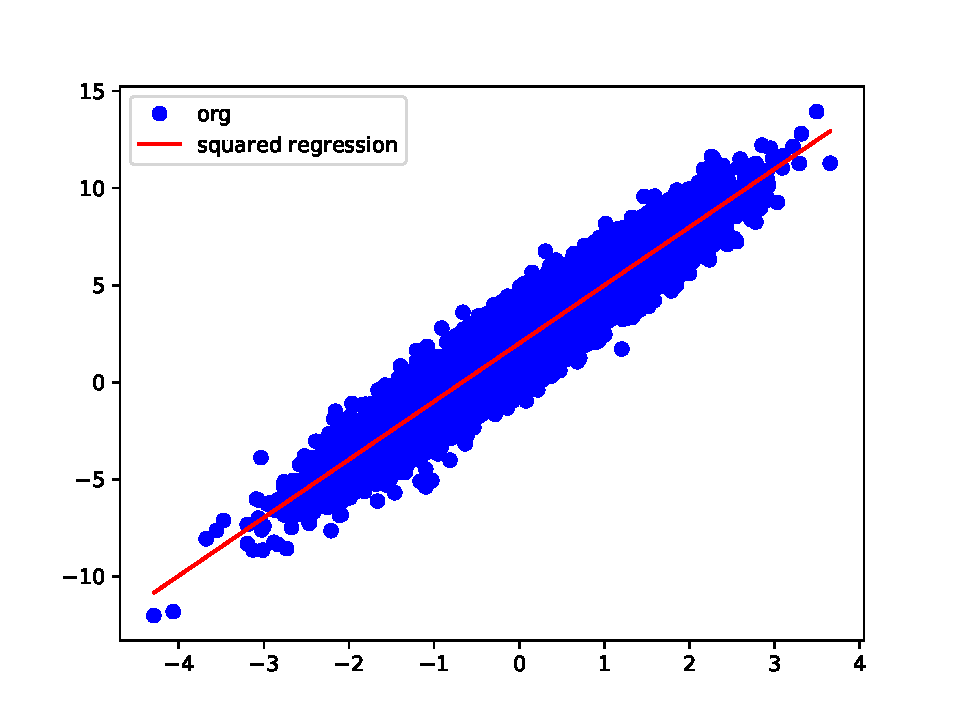
\includegraphics[scale=0.5]{imgs/squared.pdf}
  \caption{Squared loss}
  \label{squared_loss_fuc}
\end{figure}

\begin{figure}
  \centering
  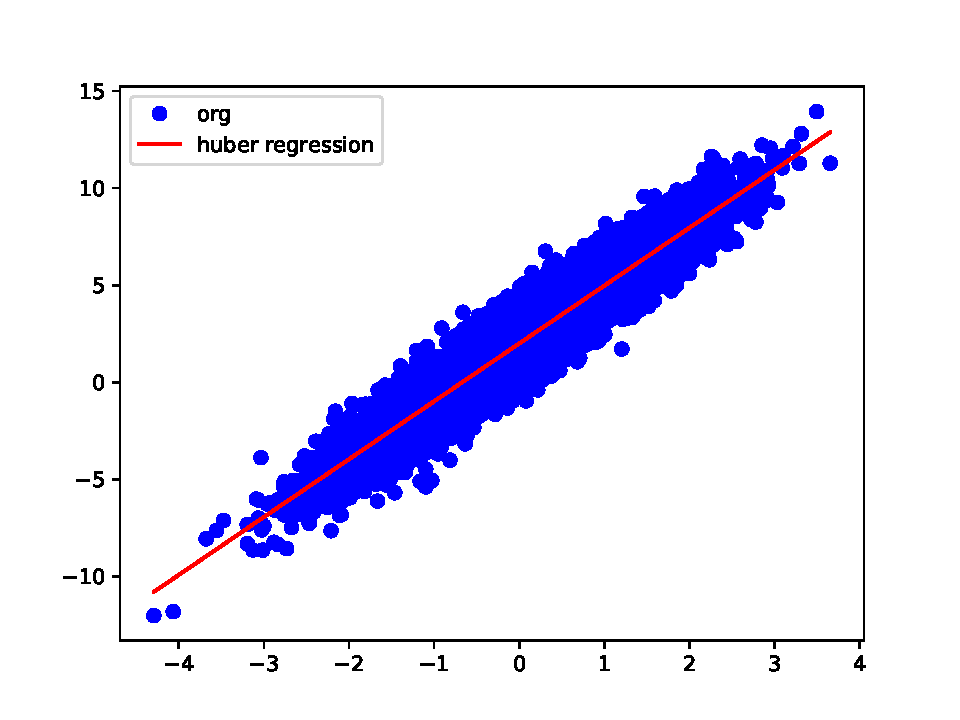
\includegraphics[scale=0.5]{imgs/huber.pdf}
  \caption{Huber loss}
  \label{huber_loss_fuc}
\end{figure}

\begin{figure}
  \centering
  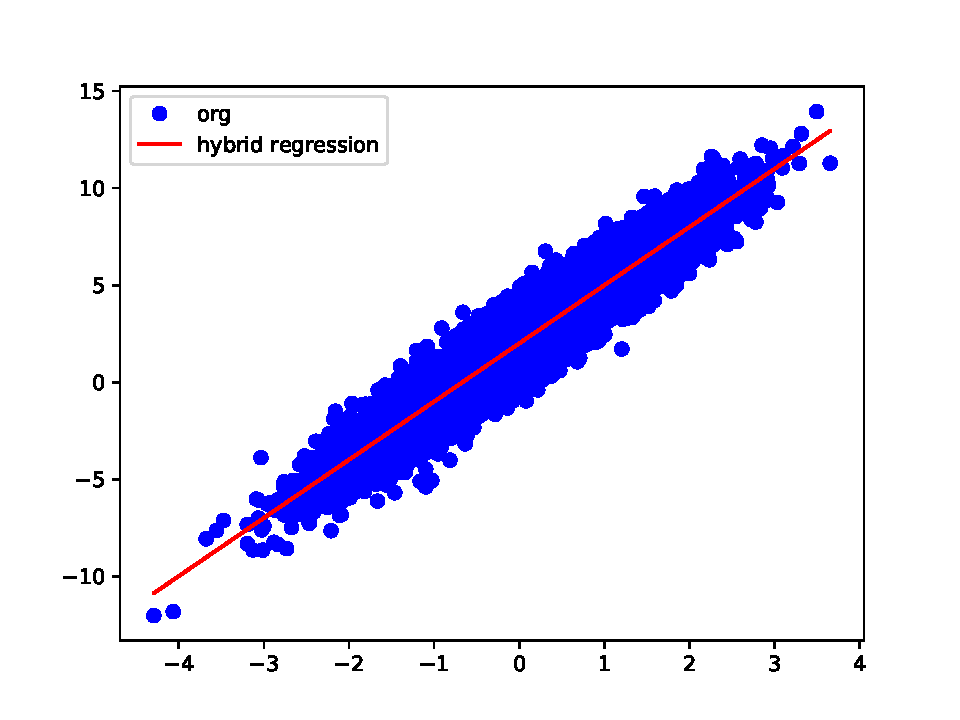
\includegraphics[scale=0.5]{imgs/hybrid.pdf}
  \caption{Hybrid loss}
  \label{hybrid_loss}
\end{figure}

\begin{figure}
  \centering
  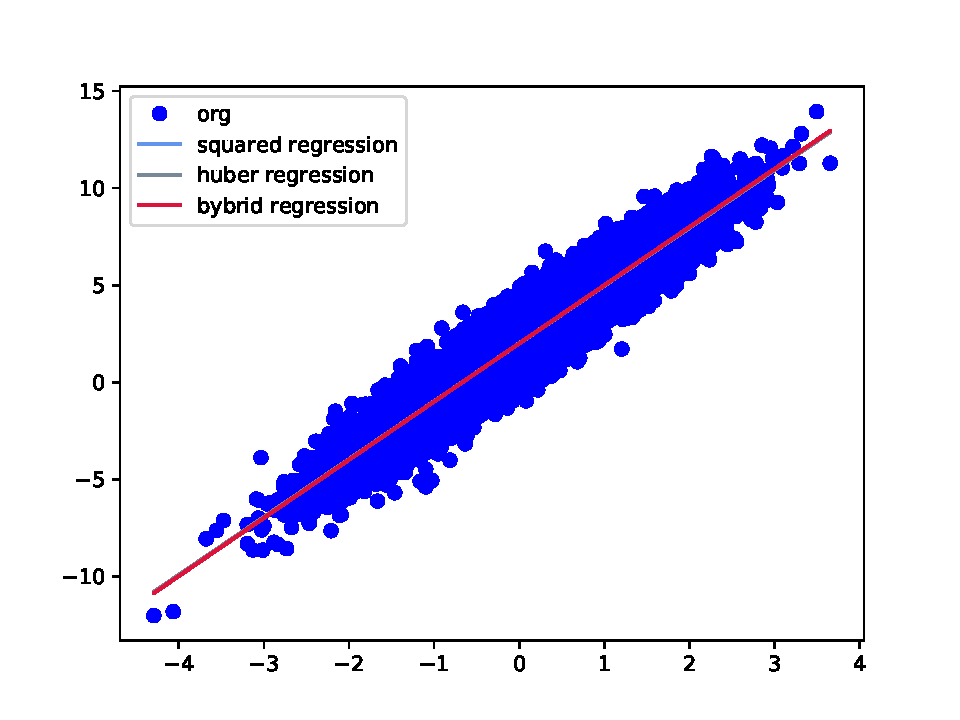
\includegraphics[scale=0.5]{imgs/all.pdf}
  \caption{Performance of different loss}
  \label{all_loss}
\end{figure}


\subsection{Learning rate}

I implemented patience scheduling. Then I tested learning rate from 0.001 to 0.01 with the incrementation 0.002, Shown in Figure \ref{lr}. The result are quite similar. Table \ref{tab:lr} shows the parameters learned under different learning rate with patience scheduling.

\begin{figure}
  \centering
  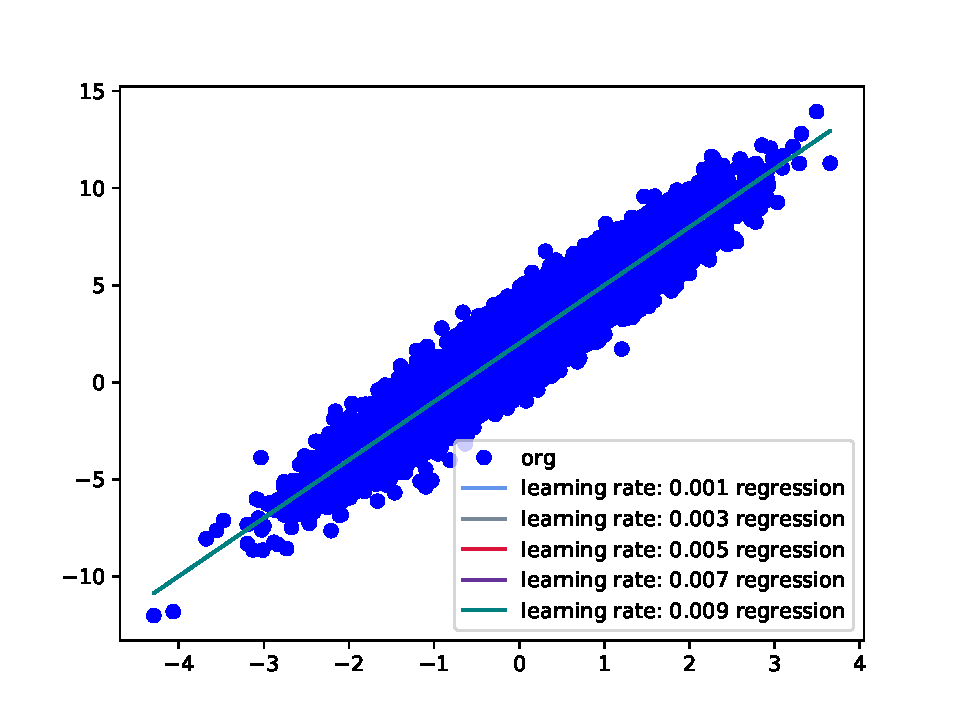
\includegraphics[scale=0.5]{imgs/lr.pdf}
  \caption{Learning rate}
  \label{lr}
\end{figure}

\begin{table}
  \caption{The performance of different learning rate}
  \label{tab:lr}
  \centering
  \begin{tabular}{lll}
    \toprule
    Learning rate     & W     & b \\
    \midrule
    0.001 & 2.9962702  & 2.0017185     \\
    0.003     & 2.9964287 & 2.001716     \\
    0.005     & 2.996503       & 2.0016577  \\
    0.007     & 2.996541 & 2.001543      \\
    0.009     & 2.9966085      & 2.0013998  \\
    \bottomrule
  \end{tabular}
\end{table}

\subsection{Training steps}
I've tested different training steps from 500 to 1500 with the incrementation 200. Shown in Figure \ref{ts}. With longer duration, the performance tend to be better. However, after "enough" steps, this effects start to stabilize and even decrease(see Table \ref{tab:ts}).

\begin{table}
  \caption{The performance of different training steps}
  \label{tab:ts}
  \centering
  \begin{tabular}{lll}
    \toprule
    Training steps     & W     & b \\
    \midrule
    500 & 2.9877446  & 1.9952948     \\
    700     & 2.995941 & 2.001462     \\
    900     & 2.9962356       & 2.0016909  \\
    1100     & 2.9962835 & 2.001727      \\
    1300    & 2.9962983      & 2.0017405  \\
    \bottomrule
  \end{tabular}
\end{table}

\begin{figure}
  \centering
  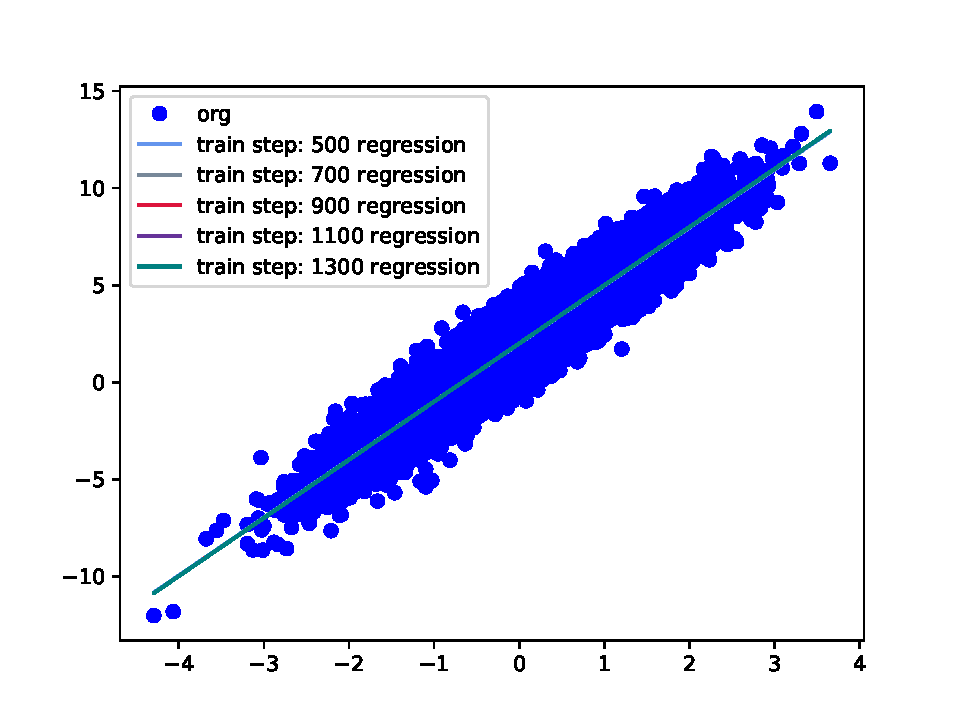
\includegraphics[scale=0.5]{imgs/ts.pdf}
  \caption{Training steps}
  \label{ts}
\end{figure}

\subsection{Initial Value of parameters}
Table \ref{tab:w} and Table \ref{tab:b} respectively denote predicted parameters with different initial parameter W and b(both of them are from -1000 to 1000 with the incrementation 500).

If I initialize the parameter W with a small number like -1000 with hybrid Loss, the predicted parameter W will become -984.0698 after 1000 epochs. That is because the model has not yet converged after 1000 epochs.

\begin{table}
  \caption{The performance of different W after 1000 epochs}
  \label{tab:w}
  \centering
  \begin{tabular}{lll}
    \toprule
    Initial W     & W     & b  \\
    \midrule
    -1000 & -984.0698 & -0.16686472    \\
    -500     & -484.0088 & -0.12897438     \\
    0     & 2.9962702      & 2.0017185  \\
    500     & 484.0088 & 0.2609221     \\
    1000    & 984.0698     & 0.22580884  \\
    \bottomrule
  \end{tabular}
\end{table}

\begin{table}
  \caption{The performance of different b after 1000 epochs}
  \label{tab:b}
  \centering
  \begin{tabular}{lll}
    \toprule
    Initial b     & W     & b  \\
    \midrule
    -1000 & -0.19055721  & -979.8584     \\
    -500     & -0.19055721 & -479.8584     \\
    0     & 2.9962702       & 2.0017185  \\
    500     & 0.19055721 & 479.8584      \\
    1000    & 0.19055721     & 979.8584  \\
    \bottomrule
  \end{tabular}
\end{table}

\subsection{Noise in data}
Before this section, I generated noise in data using normal distribution. Table \ref{noise} shows the results of different noise distribution. The distribution of noise can affect the prediction. Table \ref{normal1} shows the results of normal distribution with different mean. Table \ref{normal2} shows the results of normal distribution with different std. The level of noise is higher, the model is harder to converge.

\begin{table}
  \caption{The performance of different noise in data}
  \label{noise}
  \centering
  \begin{tabular}{lll}
    \toprule
    Noise distribution     & W     & b  \\
    \midrule
    normal(mean=0.0, stddev=1.0)     & 2.9794447 & 1.9967409    \\
    gamma(alpha=1)    & 2.98501      & 2.8410964  \\
    uniform(minval=0)    &2.9989622  &2.502729\\
    \bottomrule
  \end{tabular}
\end{table}

\begin{table}
  \caption{The performance of normal distribution with different mean}
  \label{normal1}
  \centering
  \begin{tabular}{lll}
    \toprule
    mean    & W     & b  \\
    \midrule
    0.0     & 2.9794447 & 1.9967409    \\
    1.0    & 2.964156 & 2.990973  \\
    2.0    &2.9483728 &3.9745786\\
    3.0    &2.924222 &4.9402742\\
    \bottomrule
  \end{tabular}
\end{table}

\begin{table}
  \caption{The performance of normal distribution with different std}
  \label{normal2}
  \centering
  \begin{tabular}{lll}
    \toprule
    mean    & W     & b  \\
    \midrule
    1.0    & 2.9794447 & 1.9967409 \\
    2.0    &2.8706882 &1.9283952\\
    3.0    &2.6891909 &1.8024324\\
    \bottomrule
  \end{tabular}
\end{table}

\subsection{Style}

Papers to be submitted to NeurIPS 2019 must be prepared according to the
instructions presented here. Papers may only be up to eight pages long,
including figures. Additional pages \emph{containing only acknowledgments and/or
  cited references} are allowed. Papers that exceed eight pages of content
(ignoring references) will not be reviewed, or in any other way considered for
presentation at the conference.

The margins in 2019 are the same as since 2007, which allow for $\sim$$15\%$
more words in the paper compared to earlier years.

Authors are required to use the NeurIPS \LaTeX{} style files obtainable at the
NeurIPS website as indicated below. Please make sure you use the current files
and not previous versions. Tweaking the style files may be grounds for
rejection.

\subsection{Retrieval of style files}

The style files for NeurIPS and other conference information are available on
the World Wide Web at
\begin{center}
  \url{http://www.neurips.cc/}
\end{center}
The file \verb+neurips_2019.pdf+ contains these instructions and illustrates the
various formatting requirements your NeurIPS paper must satisfy.

The only supported style file for NeurIPS 2019 is \verb+neurips_2019.sty+,
rewritten for \LaTeXe{}.  \textbf{Previous style files for \LaTeX{} 2.09,
  Microsoft Word, and RTF are no longer supported!}

The \LaTeX{} style file contains three optional arguments: \verb+final+, which
creates a camera-ready copy, \verb+preprint+, which creates a preprint for
submission to, e.g., arXiv, and \verb+nonatbib+, which will not load the
\verb+natbib+ package for you in case of package clash.

\paragraph{Preprint option}
If you wish to post a preprint of your work online, e.g., on arXiv, using the
NeurIPS style, please use the \verb+preprint+ option. This will create a
nonanonymized version of your work with the text ``Preprint. Work in progress.''
in the footer. This version may be distributed as you see fit. Please \textbf{do
  not} use the \verb+final+ option, which should \textbf{only} be used for
papers accepted to NeurIPS.

At submission time, please omit the \verb+final+ and \verb+preprint+
options. This will anonymize your submission and add line numbers to aid
review. Please do \emph{not} refer to these line numbers in your paper as they
will be removed during generation of camera-ready copies.

The file \verb+neurips_2019.tex+ may be used as a ``shell'' for writing your
paper. All you have to do is replace the author, title, abstract, and text of
the paper with your own.

The formatting instructions contained in these style files are summarized in
Sections \ref{gen_inst}, \ref{headings}, and \ref{others} below.

\section{General formatting instructions}
\label{gen_inst}

The text must be confined within a rectangle 5.5~inches (33~picas) wide and
9~inches (54~picas) long. The left margin is 1.5~inch (9~picas).  Use 10~point
type with a vertical spacing (leading) of 11~points.  Times New Roman is the
preferred typeface throughout, and will be selected for you by default.
Paragraphs are separated by \nicefrac{1}{2}~line space (5.5 points), with no
indentation.

The paper title should be 17~point, initial caps/lower case, bold, centered
between two horizontal rules. The top rule should be 4~points thick and the
bottom rule should be 1~point thick. Allow \nicefrac{1}{4}~inch space above and
below the title to rules. All pages should start at 1~inch (6~picas) from the
top of the page.

For the final version, authors' names are set in boldface, and each name is
centered above the corresponding address. The lead author's name is to be listed
first (left-most), and the co-authors' names (if different address) are set to
follow. If there is only one co-author, list both author and co-author side by
side.

Please pay special attention to the instructions in Section \ref{others}
regarding figures, tables, acknowledgments, and references.

\section{Headings: first level}
\label{headings}

All headings should be lower case (except for first word and proper nouns),
flush left, and bold.

First-level headings should be in 12-point type.

\subsection{Headings: second level}

Second-level headings should be in 10-point type.

\subsubsection{Headings: third level}

Third-level headings should be in 10-point type.

\paragraph{Paragraphs}

There is also a \verb+\paragraph+ command available, which sets the heading in
bold, flush left, and inline with the text, with the heading followed by 1\,em
of space.

\section{Citations, figures, tables, references}
\label{others}

These instructions apply to everyone.

\subsection{Citations within the text}

The \verb+natbib+ package will be loaded for you by default.  Citations may be
author/year or numeric, as long as you maintain internal consistency.  As to the
format of the references themselves, any style is acceptable as long as it is
used consistently.

The documentation for \verb+natbib+ may be found at
\begin{center}
  \url{http://mirrors.ctan.org/macros/latex/contrib/natbib/natnotes.pdf}
\end{center}
Of note is the command \verb+\citet+, which produces citations appropriate for
use in inline text.  For example,
\begin{verbatim}
   \citet{hasselmo} investigated\dots
\end{verbatim}
produces
\begin{quote}
  Hasselmo, et al.\ (1995) investigated\dots
\end{quote}

If you wish to load the \verb+natbib+ package with options, you may add the
following before loading the \verb+neurips_2019+ package:
\begin{verbatim}
   \PassOptionsToPackage{options}{natbib}
\end{verbatim}

If \verb+natbib+ clashes with another package you load, you can add the optional
argument \verb+nonatbib+ when loading the style file:
\begin{verbatim}
   \usepackage[nonatbib]{neurips_2019}
\end{verbatim}

As submission is double blind, refer to your own published work in the third
person. That is, use ``In the previous work of Jones et al.\ [4],'' not ``In our
previous work [4].'' If you cite your other papers that are not widely available
(e.g., a journal paper under review), use anonymous author names in the
citation, e.g., an author of the form ``A.\ Anonymous.''

\subsection{Footnotes}

Footnotes should be used sparingly.  If you do require a footnote, indicate
footnotes with a number\footnote{Sample of the first footnote.} in the
text. Place the footnotes at the bottom of the page on which they appear.
Precede the footnote with a horizontal rule of 2~inches (12~picas).

Note that footnotes are properly typeset \emph{after} punctuation
marks.\footnote{As in this example.}

\subsection{Figures}

\begin{figure}
  \centering
  \fbox{\rule[-.5cm]{0cm}{4cm} \rule[-.5cm]{4cm}{0cm}}
  \caption{Sample figure caption.}
\end{figure}

All artwork must be neat, clean, and legible. Lines should be dark enough for
purposes of reproduction. The figure number and caption always appear after the
figure. Place one line space before the figure caption and one line space after
the figure. The figure caption should be lower case (except for first word and
proper nouns); figures are numbered consecutively.

You may use color figures.  However, it is best for the figure captions and the
paper body to be legible if the paper is printed in either black/white or in
color.

\subsection{Tables}

All tables must be centered, neat, clean and legible.  The table number and
title always appear before the table.  See Table~\ref{sample-table}.

Place one line space before the table title, one line space after the
table title, and one line space after the table. The table title must
be lower case (except for first word and proper nouns); tables are
numbered consecutively.

Note that publication-quality tables \emph{do not contain vertical rules.} We
strongly suggest the use of the \verb+booktabs+ package, which allows for
typesetting high-quality, professional tables:
\begin{center}
  \url{https://www.ctan.org/pkg/booktabs}
\end{center}
This package was used to typeset Table~\ref{sample-table}.

\begin{table}
  \caption{Sample table title}
  \label{sample-table}
  \centering
  \begin{tabular}{lll}
    \toprule
    \multicolumn{2}{c}{Part}                   \\
    \cmidrule(r){1-2}
    Name     & Description     & Size ($\mu$m) \\
    \midrule
    Dendrite & Input terminal  & $\sim$100     \\
    Axon     & Output terminal & $\sim$10      \\
    Soma     & Cell body       & up to $10^6$  \\
    \bottomrule
  \end{tabular}
\end{table}

\section{Final instructions}

Do not change any aspects of the formatting parameters in the style files.  In
particular, do not modify the width or length of the rectangle the text should
fit into, and do not change font sizes (except perhaps in the
\textbf{References} section; see below). Please note that pages should be
numbered.

\section{Preparing PDF files}

Please prepare submission files with paper size ``US Letter,'' and not, for
example, ``A4.''

Fonts were the main cause of problems in the past years. Your PDF file must only
contain Type 1 or Embedded TrueType fonts. Here are a few instructions to
achieve this.

\begin{itemize}

\item You should directly generate PDF files using \verb+pdflatex+.

\item You can check which fonts a PDF files uses.  In Acrobat Reader, select the
  menu Files$>$Document Properties$>$Fonts and select Show All Fonts. You can
  also use the program \verb+pdffonts+ which comes with \verb+xpdf+ and is
  available out-of-the-box on most Linux machines.

\item The IEEE has recommendations for generating PDF files whose fonts are also
  acceptable for NeurIPS. Please see
  \url{http://www.emfield.org/icuwb2010/downloads/IEEE-PDF-SpecV32.pdf}

\item \verb+xfig+ "patterned" shapes are implemented with bitmap fonts.  Use
  "solid" shapes instead.

\item The \verb+\bbold+ package almost always uses bitmap fonts.  You should use
  the equivalent AMS Fonts:
\begin{verbatim}
   \usepackage{amsfonts}
\end{verbatim}
followed by, e.g., \verb+\mathbb{R}+, \verb+\mathbb{N}+, or \verb+\mathbb{C}+
for $\mathbb{R}$, $\mathbb{N}$ or $\mathbb{C}$.  You can also use the following
workaround for reals, natural and complex:
\begin{verbatim}
   \newcommand{\RR}{I\!\!R} %real numbers
   \newcommand{\Nat}{I\!\!N} %natural numbers
   \newcommand{\CC}{I\!\!\!\!C} %complex numbers
\end{verbatim}
Note that \verb+amsfonts+ is automatically loaded by the \verb+amssymb+ package.

\end{itemize}

If your file contains type 3 fonts or non embedded TrueType fonts, we will ask
you to fix it.

\subsection{Margins in \LaTeX{}}

Most of the margin problems come from figures positioned by hand using
\verb+\special+ or other commands. We suggest using the command
\verb+\includegraphics+ from the \verb+graphicx+ package. Always specify the
figure width as a multiple of the line width as in the example below:
\begin{verbatim}
   \usepackage[pdftex]{graphicx} ...
   \includegraphics[width=0.8\linewidth]{myfile.pdf}
\end{verbatim}
See Section 4.4 in the graphics bundle documentation
(\url{http://mirrors.ctan.org/macros/latex/required/graphics/grfguide.pdf})

A number of width problems arise when \LaTeX{} cannot properly hyphenate a
line. Please give LaTeX hyphenation hints using the \verb+\-+ command when
necessary.

\subsubsection*{Acknowledgments}

Use unnumbered third level headings for the acknowledgments. All acknowledgments
go at the end of the paper. Do not include acknowledgments in the anonymized
submission, only in the final paper.

\section*{References}

References follow the acknowledgments. Use unnumbered first-level heading for
the references. Any choice of citation style is acceptable as long as you are
consistent. It is permissible to reduce the font size to \verb+small+ (9 point)
when listing the references. {\bf Remember that you can use more than eight
  pages as long as the additional pages contain \emph{only} cited references.}
\medskip

\small

[1] Alexander, J.A.\ \& Mozer, M.C.\ (1995) Template-based algorithms for
connectionist rule extraction. In G.\ Tesauro, D.S.\ Touretzky and T.K.\ Leen
(eds.), {\it Advances in Neural Information Processing Systems 7},
pp.\ 609--616. Cambridge, MA: MIT Press.

[2] Bower, J.M.\ \& Beeman, D.\ (1995) {\it The Book of GENESIS: Exploring
  Realistic Neural Models with the GEneral NEural SImulation System.}  New York:
TELOS/Springer--Verlag.

[3] Hasselmo, M.E., Schnell, E.\ \& Barkai, E.\ (1995) Dynamics of learning and
recall at excitatory recurrent synapses and cholinergic modulation in rat
hippocampal region CA3. {\it Journal of Neuroscience} {\bf 15}(7):5249-5262.

\end{document}
